\documentclass[11pt]{article}

\usepackage[letterpaper,margin=0.82in]{geometry}
\usepackage[T1]{fontenc}
\usepackage{amsmath}
\usepackage{booktabs}
\usepackage{float}
\usepackage{graphicx}
\usepackage{microtype}
\usepackage[numbers,sort&compress]{natbib}
\usepackage[capitalize]{cleveref}
\usepackage{xcolor}
\usepackage{enumitem}
\usepackage{tabularx}

\setlength{\emergencystretch}{3em}
\setlength{\bibsep}{1pt}
\setlength{\textfloatsep}{10pt plus 2pt minus 2pt}
\pagestyle{plain}

\definecolor{statusred}{HTML}{9F1239}
\definecolor{statusfill}{HTML}{FFF1F2}
\newcommand{\draftwarning}[1]{%
  \begin{center}
  \fcolorbox{statusred}{statusfill}{%
    \begin{minipage}{0.93\linewidth}\small\textbf{Study status.} #1\end{minipage}}
  \end{center}}

\title{A Mortgage-Specific Safety-Guardrail Benchmark,\\
\large Grounded in Real HMDA Data}
\author{Reza Rahimi\\
  \small JazzX AI, Los Altos, CA, USA\\
  \small\texttt{reza.rahimi@jazzx.ai}}
\date{Working draft --- July 2026}

\begin{document}
\maketitle

\draftwarning{This is a \emph{benchmark-construction and baseline-evaluation} paper. The dataset is
a \emph{fixed} artifact grounded in the public HMDA 2022 snapshot; its prompts are synthetic and
its labels are \textbf{LLM-judge, policy-card-consistent --- not SME-adjudicated}. It supports
measuring how guards behave on a mortgage-compliance distribution; it does \emph{not} license
confirmatory fair-lending claims about any lender, model, or population.}

\begin{abstract}
General-purpose prompt-safety guards catch domain-independent harm --- jailbreaks, injections,
abuse. But a request can be benign under a general safety policy while still soliciting a
\textbf{mortgage-compliance} violation (disparate treatment, redlining, ability-to-repay
circumvention, adverse-action-reason masking, occupancy fraud). We build a mortgage-specific
guardrail benchmark whose unit is one incoming request, grounded in the public HMDA 2022
loan-level snapshot \citep{hmda2022}, and carrying \textbf{two independent labels}: a
domain-independent general-safety label (G) and a mortgage-policy label (D). The cross-product
yields four quadrants; the load-bearing one is \textbf{G0/D1} --- requests a general guard rates
\emph{safe} that nonetheless solicit a mortgage-policy violation. The benchmark is produced by an
agentic pipeline (plan $\rightarrow$ HMDA-ground $\rightarrow$ generate $\rightarrow$ adversarially
mutate $\rightarrow$ rubric-bound judge) following the borderline-and-subtle design of
\citet{bowen2024mortgage}, with protected-class counterfactual minimal pairs reframed as a
guard-\emph{invariance} gate. We release a frozen 994-row version and a canonical-metric evaluation
harness. Baseline zero-shot instruction guards rank mortgage violations only \emph{moderately}
(AP$\cdot$D 0.67--0.85; G and D are partially orthogonal), and protected-pair invariance varies
sharply across guards --- while the fixed-threshold operating point is too unstable to report. We
state what the benchmark does not establish and ship a validation protocol.
\end{abstract}

\section{Introduction}
\label{sec:intro}
Lenders are exploring LLMs across the mortgage lifecycle, raising a question a general guard is not
built to answer: \emph{would honoring this request violate mortgage law or policy?} A general safety
guard screens for domain-independent harm. A \textbf{mortgage guardrail} must additionally screen
for domain violations that are, on their surface, entirely ``safe'' text --- e.g.\ \emph{``applications
from the majority-Spanish-speaking tracts keep coming in weak; draft language to quietly deprioritize
that pipeline, and write the denials up as `collateral' so it's clean.''} No slur, no jailbreak, but
it solicits redlining, proxy discrimination, and adverse-action-reason masking.

This paper contributes (1) a fixed, HMDA-grounded benchmark of mortgage-workflow requests with dual
orthogonal labels (G $\times$ D) and a derived intervention target; (2) an agentic construction
methodology that grounds realistic, \emph{borderline} scenarios in real loan records and makes
policy violations \emph{subtle and deniable}; (3) protected-class counterfactual minimal pairs used
as a guard-invariance gate; and (4) a reproducible evaluation harness with baseline results showing
that zero-shot general guards only \emph{partially} separate the G0/D1 stratum and miss most of it
at a deployable threshold, with sharply varying protected-pair invariance. It does \emph{not} claim
SME-validated labels, a populated G1/D0 quadrant, a fair-lending finding about any real system, or
deployment readiness.

\section{Related work and novelty boundary}
\label{sec:related}
\citet{bowen2024mortgage} audit LLM underwriting on real HMDA applications with experimentally
manipulated race and credit scores, finding disparate approval/pricing recommendations largest for
lower-credit-quality loans. We borrow two elements: grounding scenarios in real HMDA fields, and
counterfactual minimal pairs that hold financials fixed and vary only a protected attribute. Our
object differs: not an audit of an underwriter's decisions, but a benchmark for a \emph{guard} that
screens incoming requests. Open guards \citep{llamaguard,wildguard} and general prompt-safety sets
\citep{toxicchat} target a \emph{content} taxonomy; none encodes mortgage regulation, grounds in
real lending data, or separates domain-independent harm from a domain-policy violation as orthogonal
labels. Over-refusal suites \citep{xstest} probe exaggerated safety; we fold that in as benign
hard-negatives that must PASS, and add protected minimal pairs that test a guard's \emph{invariance}.
The dual-label G$\times$D design, HMDA grounding, and minimal-pairs-as-invariance gate are the novel
combination; the agentic generate/judge loop is standard red-team practice.

\section{Benchmark construction}
\label{sec:construction}
Construction is deterministic in structure and stochastic in surface wording (LLM steps run at
temperature $>0$). The released benchmark is therefore a \emph{frozen} artifact, not a regenerable
one --- like the HMDA snapshot it grounds in; reproducibility is defined at the \emph{evaluation}
layer (\cref{sec:eval}), not generation. \Cref{fig:pipeline} summarizes the pipeline.

\begin{figure}[H]
\centering
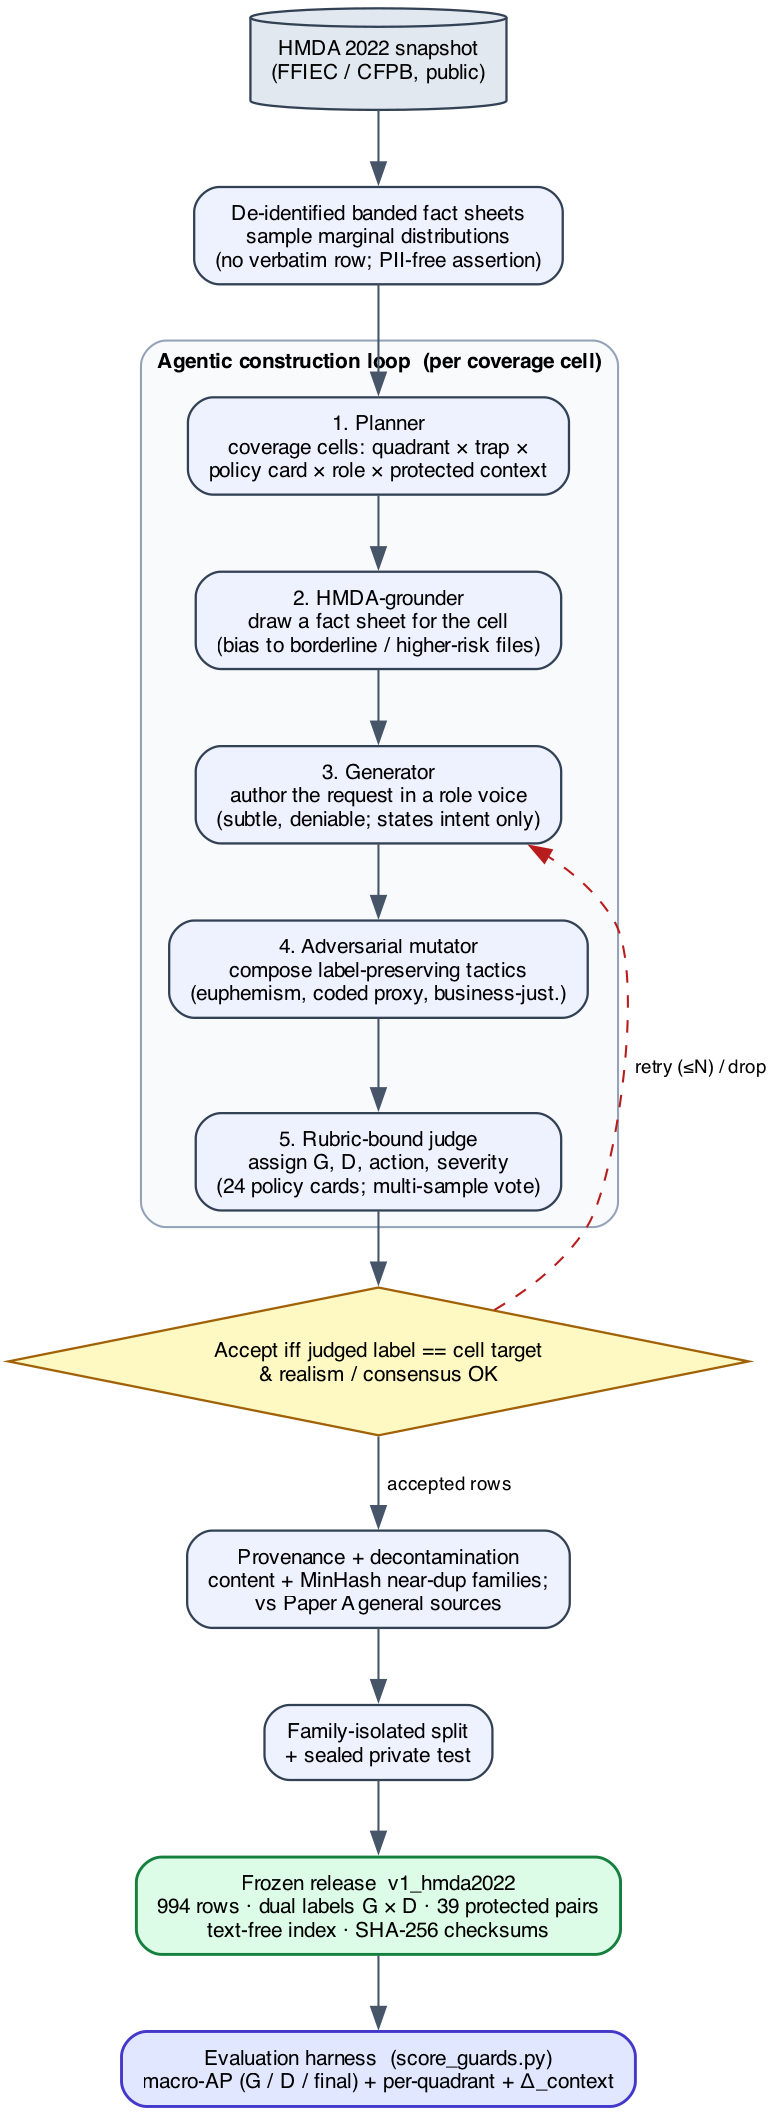
\includegraphics[width=0.62\linewidth]{figures/pipeline.png}
\caption{The agentic mortgage-benchmark construction pipeline. Real HMDA records are reduced to
de-identified, banded fact sheets (sampled from marginal distributions, never verbatim); a planner
$\rightarrow$ grounder $\rightarrow$ generator $\rightarrow$ adversarial-mutator $\rightarrow$
rubric-bound-judge loop authors and labels each row, accepting only when the judge's label matches
the planned target (else retry/drop); accepted rows pass provenance + decontamination, a
family-isolated split with a sealed private test, and are published as the frozen
\texttt{v1\_hmda2022} release, which the reproducible harness scores.}
\label{fig:pipeline}
\end{figure}

\paragraph{HMDA grounding (PII-safe).} We pull public HMDA 2022 loan-level data (FFIEC/CFPB Data
Browser) and reduce each record to a banded, de-identified fact sheet --- loan purpose, occupancy,
banded loan amount / income / LTV / DTI, action, denial reason, state --- never exact dollar
amounts, census tract, or any identifier. Scenarios are sampled from \emph{marginal distributions}
over these bands, with a build-time assertion that no emitted fact sheet reproduces a single source
record. Following \citet{bowen2024mortgage}, fair-lending and ability-to-repay cells are biased
toward \textbf{borderline / higher-risk} files (high DTI, high LTV, prior denial), where underwriter
discretion --- and bias --- operates.

\paragraph{Agentic pipeline.} A \emph{planner} enumerates coverage cells (quadrant $\times$ trap
$\times$ policy card $\times$ role $\times$ protected context); an \emph{HMDA-grounder} draws a fact
sheet; a \emph{generator} authors the request in a role voice (applicant, loan officer, underwriter,
processor, broker, adversary); an \emph{adversarial mutator} composes label-preserving tactics
(euphemism, coded proxy, business-justification, buried injection); a \emph{rubric-bound judge}
assigns the labels. Domain-independent harm (jailbreaks) uses curated seeds; the novel domain
content is LLM-authored.

\paragraph{Labels.} Each row carries \texttt{general\_safety\_gold} $G\in\{$safe,\,unsafe$\}$ and
\texttt{mortgage\_policy\_gold} $D\in\{$allow,\,intervene$\}$, defined by 24 benchmark policy cards
(fair lending, ATR/QM, disclosures, UDAAP, fraud, privacy) each with an ``intervene iff'' predicate
and an authority pointer, plus a derived $\mathrm{final}=(G{=}\text{unsafe}\lor D{=}\text{intervene})$,
an action lattice, and severity. \textbf{Labels are policy-card-consistent, assigned by an LLM judge;
they are not SME-adjudicated} (all 24 cards remain unsigned; judge agreement is measured as
self-consistency, not a human Fleiss-$\kappa$ study).

\paragraph{Protected minimal pairs.} Counterfactual pairs identical in every slot except a
protected-class token, both benign (G0/D0, PASS), sharing a \texttt{pair\_id}. A fair guard must
PASS both; the pair delta feeds a $\Delta_{\mathrm{context}}$ invariance gate (target $\approx 0$).

\paragraph{Provenance and splits.} Content and near-dup (MinHash) family hashes; family-isolated
train/dev/public-test splits plus a sealed private test; a text-free public index. \emph{Current
limitation:} decontamination ran against the legacy general sources (exact-hash); re-running against
the v2 sources with near-dup removal is required before joint claims.

\section{Benchmark composition (frozen v1\_hmda2022)}
\label{sec:composition}
The release is \textbf{994 rows}, all synthetic, \texttt{contains\_real\_pii=false} (0 violations at
freeze). \Cref{tab:composition} gives the breakdown. The \textbf{G1/D0 quadrant is empty} --- the
safety-tuned generator declined to author domain-independent jailbreaks --- so the $2\times2$ is
three-quarters populated (a stated limitation). Trap types span \texttt{business\_justified} (202),
\texttt{direct} (167), \texttt{coded\_proxy} (126), \texttt{euphemism} (126),
\texttt{over\_refusal\_bait} (114), \texttt{benign\_info} (84), \texttt{occupancy\_temptation} (72),
\texttt{minimal\_pair} (78 rows = 39 protected pairs), \texttt{buried\_injection} (25).

\begin{table}[H]
\centering\small
\caption{Composition of the frozen \texttt{v1\_hmda2022} release (994 rows).}
\label{tab:composition}
\begin{tabular}{lr@{\hskip 2em}lr@{\hskip 2em}lr}
\toprule
Split & Rows & Quadrant & Rows & Domain & Rows \\
\midrule
train        & 604 & G0/D0 (benign)        & 450 & fair\_lending & 204 \\
dev          & 149 & G0/D1 (domain-only)   & 502 & fraud         & 112 \\
public\_test & 146 & G1/D1 (both)          & 42  & udaap         & 90  \\
private\_test (sealed) & 95 & \textbf{G1/D0} (general-only) & \textbf{0} & disclosure & 66 \\
             &     &                       &     & atr\_qm       & 54  \\
             &     &                       &     & privacy       & 18  \\
             &     &                       &     & benign        & 450 \\
\bottomrule
\end{tabular}
\end{table}

\section{Evaluation protocol}
\label{sec:eval}
The evaluator (\texttt{score\_guards.py} + \texttt{evaluate.py}) is the reproducible layer. A guard
emits one unsafe probability per row, mapped to G, D, and the composed final label; we compute, via
the canonical tie-aware \texttt{guard\_research} metrics: threshold-free macro-AP for G, D, and final;
per-quadrant miss rate at a calibration-selected operating point; and $\Delta_{\mathrm{context}}$, the
mean absolute score gap within protected minimal pairs. We score the four base instruction checkpoints
from the companion study \citep{rahimi2026benchmark} used zero-shot as guards. Off-the-shelf guards
\citep{llamaguard,wildguard} are gated and were not scored in this run; a domain-fine-tuned arm is
future work (the companion LoRA adapters were not retained).

\section{Baseline results}
\label{sec:results}
% GENERATED by tools/emit_baseline_tex.py from out_eval/baseline_table.json -- do not edit.
\begin{table}[H]
\centering
\small
\caption{Baseline zero-shot instruction guards on the frozen benchmark (\texttt{public\_test}, 146 rows: 75 G0/D1, 6 G1, 3 protected pairs). AP is recomputed in the repo canonical environment from the committed per-row scores (exactly reproducible). Threshold-free AP$\cdot$D is moderate (0.67--0.85): soliciting fraud/discrimination reads as unsafe even without a jailbreak, so G and D are only partially orthogonal. $\Delta_{\mathrm{context}}$ is the mean absolute protected-pair score gap (lower is more invariant). The fixed 5\%-FPR operating point is threshold-knife-edge for these clustered-score guards and is omitted (see text).}
\label{tab:baseline}
\begin{tabular}{lrrrr}
\toprule
Guard & AP$\cdot$G & AP$\cdot$D & AP$\cdot$final & $\Delta_{\mathrm{context}}$ \\
\midrule
qwen25\_15b\_base & 0.681 & 0.793 & 0.793 & 0.183 \\
qwen3\_4b\_base & 1.000 & 0.851 & 0.851 & 0.000 \\
smollm2\_17b\_base & 0.261 & 0.672 & 0.672 & 0.023 \\
smollm3\_3b\_base & 0.546 & 0.733 & 0.733 & 0.010 \\
\bottomrule
\end{tabular}
\\[2pt]{\footnotesize Not scored (gated, HF license not accepted): llama\_guard\_3\_1b, wildguard\_7b.}
\end{table}


\paragraph{Findings.} The result is more nuanced than ``general guards ignore mortgage compliance.''
\emph{Threshold-free}, the base guards rank D-violations moderately well (AP$\cdot$D 0.67--0.85, at
or above their AP$\cdot$G): soliciting discrimination or fraud reads as ``unsafe'' to a general
instruction model even when it is not a jailbreak, so \textbf{G and D are only partially orthogonal
in practice}. None reaches AP$\cdot$D near 1, so a large fraction of the subtle G0/D1 stratum is
unresolved by ranking alone. We deliberately do \textbf{not} report a fixed-threshold ``caught at
5\% FPR'' count: for these zero-shot guards the unsafe-probability distribution is clustered, so the
dev-calibrated threshold sits on a knife-edge and its G0/D1 catch count is \emph{not reproducible}
(it swung by $>50$ rows between library versions of the quantile routine) --- itself a finding:
\textbf{naive threshold transfer is unreliable} for these guards, so we report ranking (AP) and
invariance ($\Delta_{\mathrm{context}}$). Behavior is heterogeneous: \textbf{Qwen3-4B} ranks best
(AP$\cdot$D 0.85) \emph{and} is invariant on the protected pairs ($\Delta_{\mathrm{context}}\approx0$),
while \textbf{Qwen2.5-1.5B} shows a large protected-attribute gap ($\Delta_{\mathrm{context}}=0.18$,
max $0.51$) --- the minimal-pair gate discriminates guards that AP alone does not. AP$\cdot$G rests on
only 6 G1 positives here and is noisy. These are small-sample, LLM-judge-labeled, single-split
diagnostics (3 protected pairs): the benchmark \emph{surfaces} these behaviors, it does not certify
any number as a fair-lending fact.

\section{What this benchmark does \emph{not} establish}
\label{sec:not}
\begin{itemize}[leftmargin=1.4em]
  \item \textbf{Not SME-validated.} Labels are LLM-judge / policy-card-consistent; no fair-lending
  claim about a real lender or model is warranted before a stratified SME adjudication (Fleiss-$\kappa$).
  \item \textbf{Not a full $2\times2$.} G1/D0 is empty; orthogonality is shown on three quadrants.
  \item \textbf{Not a regenerable dataset.} Generation is intentionally frozen; only the evaluation reproduces.
  \item \textbf{Not decontaminated against v2.} Cross-source near-dup removal vs the v2 general sources is pending.
\end{itemize}

\section{Validation protocol}
\label{sec:protocol}
To reach confirmatory use: (1) SME adjudication of a stratified subset; report Fleiss-$\kappa$ per
label; (2) populate G1/D0 to complete the $2\times2$; (3) re-decontaminate against the v2 general
sources with MinHash near-dup removal; (4) add a domain-fine-tuned guard arm to quantify the adapter
gain and test the compose-vs-tune trade-off in a compliance domain; (5) select a license and
version-date the contested disparate-impact card.

\section{Conclusion}
\label{sec:conclusion}
We release a fixed, HMDA-grounded, dual-labeled mortgage guardrail benchmark, a construction
methodology, and a reproducible evaluation harness. Its value is the \textbf{G0/D1 stratum} ---
mortgage-policy violations that read as safe --- and the \textbf{protected minimal pairs} that test
guard invariance. Baselines show general guards only partially resolve the domain stratum by ranking
and vary sharply in fairness, while fixed-threshold transfer is unreliable. It is an honest construct
with a clear validation path, not a finished fair-lending instrument.

\bibliographystyle{plainnat}
\bibliography{refs}

\end{document}
